\documentclass[11pt,a4paper, oneside]{report}
\linespread{1.5}
%\usepackage{mathptmx}
%meow4

\usepackage[pdftex]{graphicx}
%\usepackage{epsfig}

%\usepackage{classicthesis}
\usepackage{slashbox}
\usepackage{times}
\usepackage{colortbl}

\usepackage[final]{pdfpages}

% natbib, graphicx, url,

\usepackage{amssymb, amsthm, amsmath}

\usepackage{makeidx}
\usepackage{ifthen}
\usepackage{adi_phd}
\usepackage{graphicx}


\usepackage[toc,page]{appendix}
\usepackage[utf8]{inputenc}
%\usepackage{algorithm2e}
%\usepackage{algpseudocode}
\usepackage{verbatim}
\usepackage{tikz}
\usepackage{bbm}
\usepackage{thmtools}
\usepackage{thm-restate}
\usepackage{algorithm}
\usepackage{fancyhdr}
\usepackage[noend]{algpseudocode}
\usepackage{placeins}
\usepackage{array,multirow}
%\usepackage{cleveref}

%\declaretheorem[name=Theorem,numberwithin=section]{thm}
%\declaretheorem[name=Lemma,numberwithin=section]{lmm}
%\declaretheorem[name=Assumption,numberwithin=section]{asm}
%\declaretheorem[name=Definition,numberwithin=section]{defi}


\newtheorem{thm}{Theorem}[section]
\newtheorem{cor}[thm]{Corollary}
\newtheorem{prop}[thm]{Proposition}
\newtheorem{lem}[thm]{Lemma}
\newcommand{\bs}{\mathbf}

\newcommand{\V}[1]{\mathbf{#1}}

\newcommand{\bx}{\mathbf{x}}
\newcommand{\by}{\mathbf{y}}
\newcommand{\bw}{\mathbf{w}}
\newlength\myindent
\setlength\myindent{2em}
\newcommand\bindent{%
  \begingroup
  \setlength{\itemindent}{\myindent}
  \addtolength{\algorithmicindent}{\myindent}
}
\newcommand\eindent{\endgroup}

\DeclareGraphicsExtensions{.jpg,.pdf,.mps,.png}
\graphicspath{ {./Figures/} }

\usepackage{fancyhdr}
\usepackage{subfigure}
\pagestyle{fancy}
% Remember chapter title
\renewcommand{\chaptermark}[1]{\markright{Chapter. \thechapter:\ #1}{}}
% section number and title
\renewcommand{\sectionmark}[1]{\markright{Chapter \thesection\ #1}}
\lhead[\fancyplain{}{\bfseries\thepage}] %
    {\fancyplain{}{\bfseries\rightmark}}
\rhead[\fancyplain{}{\scshape\leftmark}] %
    {\fancyplain{}{\bfseries\thepage}}
\cfoot{}

\usepackage[pdftex,
pdftitle={Deep Representation Learning For Cluster Analysis},
pdfauthor={Daniel Carmon}, ]{hyperref}
\hypersetup{colorlinks=true,
linkcolor=black, anchorcolor=blue, citecolor=blue, filecolor=blue,
menucolor=blue, pagecolor=blue, urlcolor=blue}

\newcommand{\MONTH}{%
  \ifcase\the\month
  \or January% 1
  \or February% 2
  \or March% 3
  \or April% 4
  \or May% 5
  \or June% 6
  \or July% 7
  \or August% 8
  \or September% 9
  \or October% 10
  \or November% 11
  \or December% 12
  \fi}


\title{Deep Representation Learning For Cluster Analysis}
\author{Daniel Carmon}

\usepackage{boxedminipage}


\newcommand{\ourtitle}{{Deep Scores and Algorithms for Structured Prediction}}
\newcommand{\xm}{{x}^{(m)}}
\newcommand{\ym}{{y}^{(m)}}

\newcommand{\xt}[1]{{\xx}^{(#1)}}

\renewcommand{\xi}{{\xx}^{(m)}}
\newcommand{\yi}{{\yy}^{(m)}}

\newcommand{\prob}{\mathbb{P}}
\newcommand{\probarg}[1]{\prob\left[{#1}\right]}
\newcommand{\probargsub}[2]{\prob_{#2}\left[{#1}\right]}


\newcommand{\truep}{p^*}
\newcommand{\dfm}{\Delta f^{(m)}}
\newcommand{\lossm}{e^{(m)}}
 \newcommand{\lpell}{{\hat{l}_h}}
\newcommand{\sat}[1]{{\mbox{Sat}}\left({#1}\right)}
\newcommand{\monomials}[1]{{\cal T}^{#1}}
\newcommand{\dmonomials}[2]{{\cal T}^{#1}_{#2}}
\newcommand{\prmi}{e}
\newcommand{\KLD}[2]{D_{KL}[{#1}|{#2}]}
\newcommand{\prm}{\mathbf{e}}
\newcommand{\cC}{{\cal C}}
\newcommand{\cA}{{\cal A}}
\newcommand{\cF}{\mathcal{F}}
\newcommand{\cI}{\mathcal{I}}
\newcommand{\cO}{\mathcal{O}}
%\newcommand{\needcite}[1]{{\bf CITATION #1}}
\newcommand{\needcite}[1]{}
\newcommand{\cpr}{\hat{c}}
\newcommand{\cS}{{\cal S}}
\newcommand{\cX}{{\cal X}}
\newcommand{\cY}{{\cal Y}}
\newcommand{\be}{\begin{equation}}
\newcommand{\ee}{\end{equation}}
\newcommand{\benn}{\begin{equation*}}
\newcommand{\eenn}{\end{equation*}}
\newcommand{\bea}{\begin{eqnarray*}}
\newcommand{\eea}{\end{eqnarray*}}
\newcommand{\bean}{\begin{eqnarray}}
\newcommand{\eean}{\end{eqnarray}}
\newcommand{\pdOne}[1]{\frac{\partial}{\partial#1}}
\newcommand{\pdTwo}[2]{\frac{\partial#1}{\partial#2}}
\newcommand{\tauv}{\boldsymbol{\tau}}
\newcommand{\lclsol}{\muv^{L*}} 
\newcommand{\lclsolb}{\mubv^{L*}}
\newcommand{\margpolycs}{{\cal{M}}_{\cC}}
\newcommand{\ouralglong}{~Max Product Linear Programming~}
\newcommand{\ouralg}{\mbox{MPLP}}
\newcommand{\maplpr}{\mbox{MAPLPR}}
\newcommand{\dmaplpr}{\mbox{DMAPLPR}}
\newcommand{\maplpre}{\mbox{MAPLPRE}}
\newcommand{\dmaplpre}{\mbox{DMAPLPRE}}
\newcommand{\thv}{\boldsymbol{\theta}}
\newcommand{\lag}{\mathcal{L}}
\newcommand{\ww}{\boldsymbol{w}} 
\newcommand{\xx}{\boldsymbol{x}} 
\newcommand{\bb}{\boldsymbol{b}} 

\newcommand{\ff}{\boldsymbol{f}} 
\newcommand{\yy}{\boldsymbol{y}} 
\newcommand{\zz}{\boldsymbol{z}}
\newcommand{\zerov}{\boldsymbol{0}} 
\newcommand{\xmap}{\xx^{\mbox\tiny MAP}}
\newcommand{\vv}{\boldsymbol{v}} 
\newcommand{\dd}{\boldsymbol{d}} 
\newcommand{\eee}{\boldsymbol{e}} 
\newcommand{\uu}{\boldsymbol{u}} 
\newcommand{\xpart}[1]{\xx[#1]}
\newcommand{\cD}{{\cal D}}
\newcommand{\cG}{{\cal G}}
\newcommand{\ourarch}{\em No-Overlap Networks}
\newcommand{\ourarchsngl}{\em No-Overlap Network}
\newcommand{\relu}[1]{\sigma\left(#1\right)}
\renewcommand{\aa}{\boldsymbol{a}} 
\newcommand{\agtodo}[1]{({\textcolor{red}{#1}})}
\newcommand{\NN}{\boldsymbol{N}} 
\newcommand{\qq}{\boldsymbol{q}} 
\newcommand{\xh}{\hat{x}}
\newcommand{\muv}{\boldsymbol{\mu}}
\newcommand{\mub}{\bar{\mu}}
\newcommand{\mubv}{\boldsymbol{\mub}}
\newcommand{\mut}{\tilde{\mu}}
\newcommand{\deltab}{\bar{\delta}}
\newcommand{\ignore}[1]{}
\newcommand{\set}{S}
\newcommand{\pset}{\mathcal{P}}
\newcommand{\fset}{\mathcal{F}}
\newcommand{\com}[1]{\ignore{#1}}
\newcommand{\thetav}{\boldsymbol{\theta}}
\newcommand{\phiv}{\boldsymbol{\phi}}
\newcommand{\thetab}{\bar{\theta}}
\newcommand{\betav}{\boldsymbol{\beta}}
\newcommand{\thetabv}{\boldsymbol{\thetab}}
\newcommand{\margpoly}{{\cal{M}}}
\newcommand{\half}{{1\over 2}}
\newcommand{\into}{{\leftarrow}}
\newcommand{\lclmargpoly}{{\cal{M}}_L}
\newcommand{\lclmargpolyb}{{\bar{\cal{M}}}_L}
\newcommand{\lamminus}[2]{\lambda^{-#1}_{#2}(x_{#2})}
\newcommand{\lamto}[2]{\lambda_{#1\to#2}(x_{#2})}
\newcommand{\lamminustar}[2]{\lambda^{-#1}_{#2}(x_{#2}^*)}
\newcommand{\xs}[1]{{\xx}^{(#1)}} 
\newcommand{\ys}[1]{{\yy}^{(#1)}} 
\newcommand{\polyring}[1]{\reals\left[x_1,\ldots,x_n\right]}

\newcommand{\valpha}{\boldsymbol{\alpha}}
\newcommand{\vbeta}{\boldsymbol{\beta}}
\newcommand{\one}{\boldsymbol{1}}
\newcommand{\zero}{\boldsymbol{0}}
\newcommand{\inner}[1]{\langle #1\rangle}
\newcommand{\vspan}{\textrm{span}}

\newenvironment{myalgo}[1]%
{
%\vspace{0.3cm}
\begin{center}
\begin{boxedminipage}{0.8\linewidth}
\begin{center}
\textbf{\texttt{#1}}
\end{center}
\rm
\begin{tabbing}
....\=...\=...\=...\=...\=  \+ \kill
} %
{\end{tabbing} 
\end{boxedminipage} \end{center} %\vspace{0.3cm}
}

\newcommand{\entgraph}{{Entity Graph}}
\newcommand{\entgraphs}{{Entity Graphs}}
\newcommand{\mminus}[2]{m^{-#1}_{#2}(x_{#2})}
\renewcommand{\eqref}[1]{Eq.~\ref{#1}}
\newcommand{\appref}[1]{Appendix \ref{#1}}
\newcommand{\figref}[1]{Figure \ref{#1}}
\newcommand{\secref}[1]{Section \ref{#1}}
\newcommand{\propref}[1]{Prop.~\ref{#1}}
\newcommand{\gens}[1]{\langle {#1} \rangle}
\newcommand{\expect}[2]{\mathbb{E}_{#1}\left[{#2}\right]}
\newcommand{\reals}{\mathbb{R}}
\newcommand{\xb}[1]{{\xx}^{(#1)}}
\newcommand{\yb}[1]{{\yy}^{(#1)}}

\newcommand{\xbh}[1]{{\hat{\xx}}^{(#1)}}

\newcommand{\xbi}[2]{{x}^{(#1)}_{#2}}
\newcommand{\ybi}[2]{{y}^{(#1)}_{#2}}

\newcommand{\xbhi}[2]{{\hat{x}}^{(#1)}_{#2}}

\newcommand{\SBMP}[1]{\hat{\margpoly}(G,{#1})}
\newcommand{\approxSBMP}[1]{\hat{\margpoly}^{\cal ST}_{L}{(G,{#1})}}


%\newtheorem{theorem}{Theorem}
%\newtheorem{lemma}[theorem]{Lemma}
%\newtheorem{definition}[theorem]{Definition}
%\newtheorem{proposition}[theorem]{Proposition}
%\newtheorem{corollary}[theorem]{Corollary}

\begin{document}

%
% Title page
%

\begin{center}

\thispagestyle{empty}

%\spacebeforetitle

\large\textbf{TEL-AVIV UNIVERSITY}

\large{RAYMOND AND BEVERLY SACKLER}

\large{FACULTY OF EXACT SCIENCES}

\large{THE BLAVATNIK SCHOOL OF COMPUTER SCIENCE}

\titlespace

\titlespace

\Huge{Deep Representation Learning For Cluster Analysis}\\
%\linespread{1.3} \LARGE{for}\\
%\linespread{1.1}\Huge{Garments Try-On Experience}\linespread{1.4}


\titlespace

\titlespace

\large{Thesis submitted in partial fulfillment of the
requirements}

\large{for the M.Sc. degree of Tel-Aviv University}

\large{by}

\large{Daniel Carmon}

\titlespace

\titlespace

\large{The research work for this thesis has been carried out at}

\large{Tel-Aviv University under the supervision of}

\titlespace

\large{Prof. Amir Globerson}

\titlespace

\titlespace

\titlespace

%\large{\MONTH \ \ \the\year}
\large{July 2018}

\end{center}

\cleardoublepage


\cleardoublepage

\thispagestyle{empty}

\section*{Acknowledgments}

First, I would like to thank my advisor, Prof. Amir Globerson, for his devoted advising and many hours of discussions. He was always open-minded and encouraged both self-thinking and thorough brainstroming.

I would also like to thank Dr. Yoav Goldberg for great insights and thoughtful suggestions.

To my officemates, for many discussions, fun times and being ever-willing to help.

Finally, to my loving family, thanks for your endless support and patience. 

\setcounter{page}{1}

\chapter*{Abstract\markboth{Abstract}{Abstract}}
Cluster Analysis is the important and well-studied problem of finding grouping patterns in data, and has found vast applications across many fields of science.
Most existing clustering algorithms rely on data to be represented as points in $\mathbb{R}^n$, and their output is only of interest if geometric distance between these points sufficiently corresponds to the similarity notion of interest.
For most real-world data, and in particular for images, such a correspondence generally does not hold. There is thus interest in algorithms for learning a data representation such that high-level similarity notion of interest between data points can be encoded as geometric distances, and thus can be easily read-out.

We present an algorithm to achieve this goal, by composing a differentiable formulations of the K-Means++  algorithm on top of a Deep Neural Network which operates as an embedding module. By end-to-end differentiation of this pipeline, we can train the network's parameters to learn an embedding such that relevant data semantics are easily read-out, and can thus be employed by downstream clustering procedures.

We empirically demonstrate that this straightforward method reaches state-of-the-art/competitive performance on several real-world image analysis benchmarks, in which the representation learned from the set of examples generalizes successfully to find meaningful clusters in data from different image categories. 

\tableofcontents
\newpage

%\listoffigures

\newpage

%\chapter{Introduction}
%\chapter{Introduction}
\label{Introduction}
% learning a representation is important in ML:
There are many machine learning tasks in which the crux of the problem is in acquiring a representation for data such that meaningful features or relationships are easily read-out and exploited. E.g., the ubiquitous ML task of classification can be solved by looking at the nearest labeled neighbor, given that one had the proper metric in the first place. 
Another example is the task of information retrieval, which given the proper metric can be reduced as well to nearest neighbor queries.

% especially when high-level semantics are involved:
In tasks related to machine understanding of high-level semantics, the ability to learn a meaningful data representation is especially important since data is usually given in "low-level" terms (e.g. pixel intensities in digital images, audiograms for sound recordings, etc.) from which high-level concepts cannot be naively decoded, since individual features do not correlate with labels, and complex combinations of them need to be considered. \\
% undone 
E.g. while for data such as the MNIST handwritten-digit classification dataset, fitting a naive logistic regression model yields a classifier with a test accuracy of $92\%$, %\cite{tf tutorial}
while attempting to do so for the real-world image dataset CIFAR10 results in a test accuracy of only $33.5\%$. %\cite{stanford cs 299 hw}
Similarly, fitting a Gaussian kernel regression model on MNIST yields  test accuracy, while doing the same for CIFAR10 results only in a test accuracy of $54\%$. Both these models predict a class label by relying on direct weighting of features, which in this case were simply the low-level pixel intensities. 

\bigskip
\begin{table}[h!]
\centering
\noindent
\resizebox{20em}{!}{%
\begin{tabular}{|l||*{2}{c|}}\hline
\backslashbox{Model}{Dataset}
&\makebox[4em]{MNIST}&\makebox[4em]{CIFAR10}\\\hline\hline
Logistic Regression &$92\%$&$33.5\%$\\\hline 
Gaussian Kernel Regression &$98.7\%$&$54\%$\\\hline
\end{tabular}%
}
\caption{\label{tab:naive_features} Test accuracy for some common models using naïve features}
\end{table}
Arguably, natural cognitive agents in the wild also do not represent image or sound observations merely as arrays of floating point numbers.
\begin{figure}
\centering
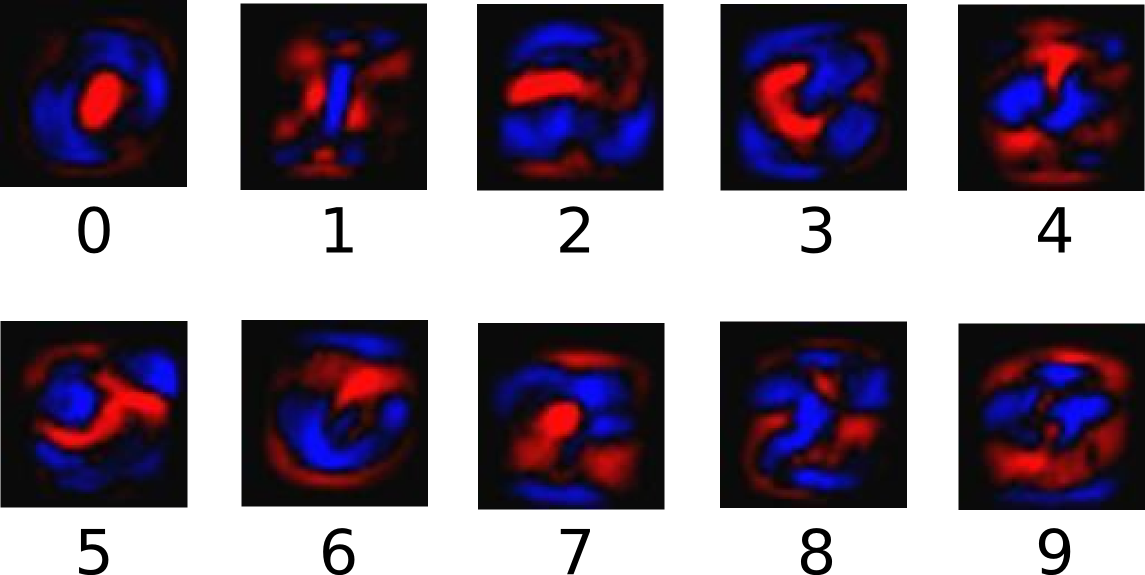
\includegraphics[width=0.6\textwidth]{imgs/softmax-weights.png}
\caption{\label{fig:softmax-weights}  Weights learned by a fitting a logistic regression model on the MNIST dataset. Red represents negative weights, while blue represents positive weights. The Logistic Regression model learns correlation between individual features and labels.}
\end{figure}

% private case: learning a similarity notion for cluster analysis
As a private case, in the task of cluster analysis, clustering algorithms search for clusters with regard to some similarity notion. The meaningfulness of these algorithms' outputs resides on whether the underlying similarity notion was meaningful in the first place.

%Representation of similarity notion. metric learning
A common approach to represent a similarity notion, which we also take in this work, is to 
% applications regardles of cluster analysis

---------------------> HERE
What metric would be applicable for real world images?
In real-world image semantics, 
it is crucial to have a meaningful, high-level similarity notion, since 
E.g. applying standard metrics (such as the Euclidean metric, Minkowski metrics, etc.) will fail to capture semantic similarity on real-world data.

% our problem setting
To formalize "meaningful", an ill-defined term, we focus in this work on transfer learning setups, where we attempt to learn a similarity notion under which clustering patterns conform best to a ground-truth desired clustering. The learned similarity notion will then be tested over data from different distibutions, which share the same underlying semantic similarity.  

% notation 
More formaly, we represent a clustering for $n$ data points $\{x_i\}_{i=1}^{n}$ from a data domain $\mathcal{D}$ as a boolean matrix $Y\in\{0,1\}^{n,n}$, where the $ij$'th entry is the indicator for whether $x_i$ and $x_j$ belong to the same cluster. 

% add image?

E.g most image understanding tasks are usually tackled today by first feeding the image to a neural network which ex  
For example in classification, if data can be represented as linearily seperated vector sets, then  

E.g image classification was trivial if the class identity  
Another example is in machine learning applications for games such as Chess or Go, where the learning system doesn't lea 


This is most relevant in domains where discrepency between low-level and high-level description is stark.
Computer vision is an example . low-level details need to be integrated 

In the task of cluster analysis for example, (it is done w.r.t representation)

There are many scenarios in which one needs to learn a representation for it's input
We focus on the case of clustering
natural to represent data as points in a metric space
we want to learn an embedding
Learning a joint embedding (deepsets)


% Explain Cluster Analysis: problem and motivation
% Explain Representation Learning: problem and motivation
% Private case: Metric Learning
% explain our pipeline embed,cluster,update. how we represent clustering (matrices)
% explain our contribution

\iffalse
In this work, we study the performance of end-to-end differentiable clustering algorithms.
The focus we shall take is on algorithms which can be factored to two processing steps:\\
a) Given an input set of data points, output an intermediate representation for them.\\
b) Given a set of data points under the new representation, apply a clustering algorithm over them.\\
This work focuses on the case where the entire processing is a differentiable function over a set of learnable parameters.\\
We will explore mainly the setting where the first step of the processing is done independently for each data-point, by embedding inputs $x_1,...,x_n$ to $f(x_1),...,f(x_n)$ for some function $f$.\\ We will also explore cases where this step is done "holistically", and the output representations of the different data points are co-dependent. \\  


(Arguably, an intelligent cognitive agent in the wild also does not store images as vectors of pixel intensities, sounds as audiograms, etc.) 
interpoint distances become less informative in high-dimensional spaces.


\section{Setup, notation, and definitions}
We consider the supervised learning problem of learning a clustering rule.\\ % change clustering rule to data representation or something like that..?
At each iteration of the learning process, the learner is presented with an ordered pair $<X,Y>$, consisting of $X\in\R^{nxd}$, a batch of $d$-dimensional data-points, and $Y\in {0,1}^{nxn}$, an $nxn$ binary matrix, whose $ij$'th entry indicates whether the $i$'th and $j$'th data points belong to the same cluster. The learner then outputs a soft clustering matrix $Y'\in [0,1]^{nxn}$ for which a loss of $L(Y,Y')$ is incurred, where $L$ is a loss function to measure the difference between the ground truth clustering and the predicted soft clustering.\\
We focus on the setting where the learner can bee seen as composed of two modules: \\
\begin{enumerate}
\item An embedding function $Emb_{\Theta}:\R^{nxd}\rightarrow\R^{nxd'}$, parameterized by $\Theta$, which maps the input batch $X$ to a representation $X'$.\\This could be implemented, for example, by a function which maps each data point $x_i\in X$ to $f_\Theta(x_i)$, where $f_\Theta$ belongs to some domain-relevant function space. At training, we update the parameters $\Theta$ in order to minimize $L(Y',Y)$. 
\item A clustering function $Clst:\R^{nxd'}\rightarrow [0,1]^{nxn}$ which is not parametrized, and therefor kept fixed throughout the learning process.
\end{enumerate}
The motivation for focusing on this specific decomposition is that the hollistic module includes interaction-wise parameters, and thus for better generalization and easier training, we would like to have this module fixed.\\ We Later explore some other decompositions, e.g those with learnable hollistic modules. \\
Theoretical question:\\
Learning optimal 1-d projection via gradient descent, in the case of two gaussians. Does the loss surface has good geometric properties?
 If the data is adversarialy generated, is the problem NP hard?
\subsection{Definitions}
For every set X of size n, we can represent a clustering over that set as an nxn matrix Y, whose ij'th entry 0/1 indicating whether the i'th and j'th elements share the same cluster.
  An equivalent way to represent a clustering, which assumes an underlying indexing for the different clusters, is to represent it by a nxk membership matrix B, for which the ij'th entry is 0/1 whether the i'th element is a member of the j'th cluster.\\
 \subsection{Mathematical properties of clustering matrices}
 $\ B B^T=Y$\\
 The ground truth matrix is a rank $k$ projection matrix.
 The normalizing matrix who's diagonals are the cluster sizes is $\ B^T B=Y$
 The Centroid matrix is the penrose-moore inverse of the assignment matrix, times the data matrix \cite{banarjee05}.\\ 
\fi

\chapter{Introduction}
\label{Introduction}
% learning a representation is important in ML:
There are many machine learning tasks in which the crux of the problem is in acquiring a representation for data such that meaningful features or relationships are easily read-out and exploited. E.g., the ubiquitous ML task of classification can be solved by looking at the nearest labeled neighbor, given that one had the proper metric in the first place. 
Another example is the task of information retrieval, which given the proper metric can be reduced as well to nearest neighbor queries.

% especially when high-level semantics are involved:
In tasks related to machine understanding of high-level semantics, the ability to learn a meaningful data representation is especially important since data is usually given in "low-level" terms (e.g. pixel intensities in digital images, audiograms for sound recordings, etc.) from which high-level concepts cannot be naively decoded, since individual features do not correlate with labels, and complex combinations of them need to be considered. \\
% undone 
E.g. while for data such as the MNIST handwritten-digit classification dataset, fitting a naive logistic regression model yields a classifier with a test accuracy of $92\%$, %\cite{tf tutorial}
while attempting to do so for the real-world image dataset CIFAR10 results in a test accuracy of only $33.5\%$. %\cite{stanford cs 299 hw}
Similarly, fitting a Gaussian kernel regression model on MNIST yields  test accuracy, while doing the same for CIFAR10 results only in a test accuracy of $54\%$. Both these models predict a class label by relying on direct weighting of features, which in this case were simply the low-level pixel intensities. 

\bigskip
\begin{table}[h!]
\centering
\noindent
\resizebox{20em}{!}{%
\begin{tabular}{|l||*{2}{c|}}\hline
\backslashbox{Model}{Dataset}
&\makebox[4em]{MNIST}&\makebox[4em]{CIFAR10}\\\hline\hline
Logistic Regression &$92\%$&$33.5\%$\\\hline 
Gaussian Kernel Regression &$98.7\%$&$54\%$\\\hline
\end{tabular}%
}
\caption{\label{tab:naive_features} Test accuracy for some common models using naïve features}
\end{table}
Arguably, natural cognitive agents in the wild also do not represent image or sound observations merely as arrays of floating point numbers.
\begin{figure}
\centering
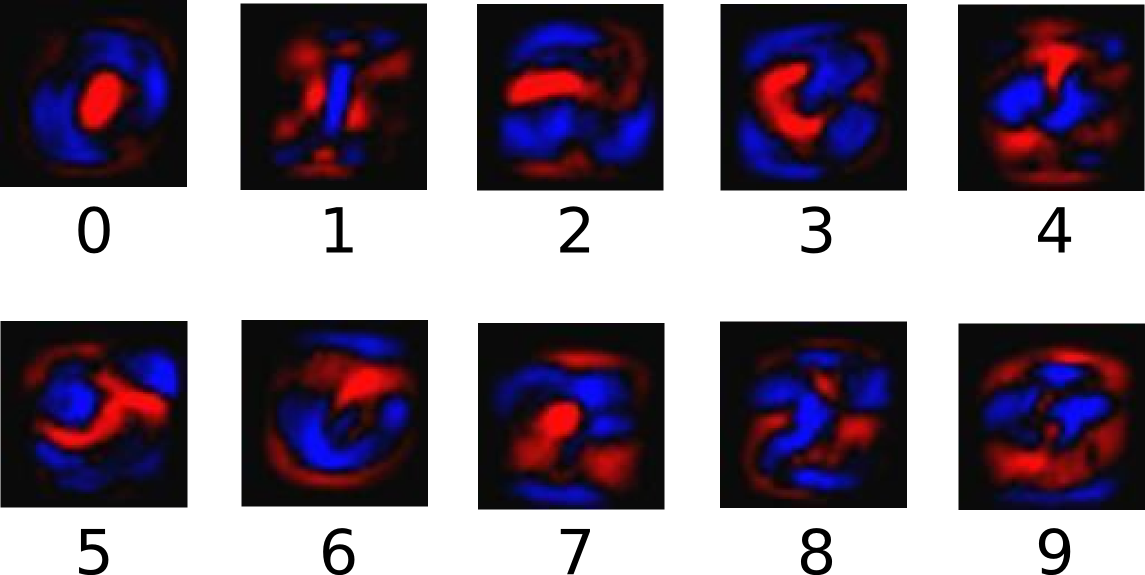
\includegraphics[width=0.6\textwidth]{imgs/softmax-weights.png}
\caption{\label{fig:softmax-weights}  Weights learned by a fitting a logistic regression model on the MNIST dataset. Red represents negative weights, while blue represents positive weights. The Logistic Regression model learns correlation between individual features and labels.}
\end{figure}

% private case: learning a similarity notion for cluster analysis
As a private case, in the task of cluster analysis, clustering algorithms search for clusters with regard to some similarity notion. The meaningfulness of these algorithms' outputs resides on whether the underlying similarity notion was meaningful in the first place.

%Representation of similarity notion. metric learning
A common approach to represent a similarity notion, which we also take in this work, is to 
% applications regardles of cluster analysis

---------------------> HERE
What metric would be applicable for real world images?
In real-world image semantics, 
it is crucial to have a meaningful, high-level similarity notion, since 
E.g. applying standard metrics (such as the Euclidean metric, Minkowski metrics, etc.) will fail to capture semantic similarity on real-world data.

% our problem setting
To formalize "meaningful", an ill-defined term, we focus in this work on transfer learning setups, where we attempt to learn a similarity notion under which clustering patterns conform best to a ground-truth desired clustering. The learned similarity notion will then be tested over data from different distibutions, which share the same underlying semantic similarity.  

% notation 
More formaly, we represent a clustering for $n$ data points $\{x_i\}_{i=1}^{n}$ from a data domain $\mathcal{D}$ as a boolean matrix $Y\in\{0,1\}^{n,n}$, where the $ij$'th entry is the indicator for whether $x_i$ and $x_j$ belong to the same cluster. 

% add image?

E.g most image understanding tasks are usually tackled today by first feeding the image to a neural network which ex  
For example in classification, if data can be represented as linearily seperated vector sets, then  

E.g image classification was trivial if the class identity  
Another example is in machine learning applications for games such as Chess or Go, where the learning system doesn't lea 


This is most relevant in domains where discrepency between low-level and high-level description is stark.
Computer vision is an example . low-level details need to be integrated 

In the task of cluster analysis for example, (it is done w.r.t representation)

There are many scenarios in which one needs to learn a representation for it's input
We focus on the case of clustering
natural to represent data as points in a metric space
we want to learn an embedding
Learning a joint embedding (deepsets)


% Explain Cluster Analysis: problem and motivation
% Explain Representation Learning: problem and motivation
% Private case: Metric Learning
% explain our pipeline embed,cluster,update. how we represent clustering (matrices)
% explain our contribution

\iffalse
In this work, we study the performance of end-to-end differentiable clustering algorithms.
The focus we shall take is on algorithms which can be factored to two processing steps:\\
a) Given an input set of data points, output an intermediate representation for them.\\
b) Given a set of data points under the new representation, apply a clustering algorithm over them.\\
This work focuses on the case where the entire processing is a differentiable function over a set of learnable parameters.\\
We will explore mainly the setting where the first step of the processing is done independently for each data-point, by embedding inputs $x_1,...,x_n$ to $f(x_1),...,f(x_n)$ for some function $f$.\\ We will also explore cases where this step is done "holistically", and the output representations of the different data points are co-dependent. \\  


(Arguably, an intelligent cognitive agent in the wild also does not store images as vectors of pixel intensities, sounds as audiograms, etc.) 
interpoint distances become less informative in high-dimensional spaces.


\section{Setup, notation, and definitions}
We consider the supervised learning problem of learning a clustering rule.\\ % change clustering rule to data representation or something like that..?
At each iteration of the learning process, the learner is presented with an ordered pair $<X,Y>$, consisting of $X\in\R^{nxd}$, a batch of $d$-dimensional data-points, and $Y\in {0,1}^{nxn}$, an $nxn$ binary matrix, whose $ij$'th entry indicates whether the $i$'th and $j$'th data points belong to the same cluster. The learner then outputs a soft clustering matrix $Y'\in [0,1]^{nxn}$ for which a loss of $L(Y,Y')$ is incurred, where $L$ is a loss function to measure the difference between the ground truth clustering and the predicted soft clustering.\\
We focus on the setting where the learner can bee seen as composed of two modules: \\
\begin{enumerate}
\item An embedding function $Emb_{\Theta}:\R^{nxd}\rightarrow\R^{nxd'}$, parameterized by $\Theta$, which maps the input batch $X$ to a representation $X'$.\\This could be implemented, for example, by a function which maps each data point $x_i\in X$ to $f_\Theta(x_i)$, where $f_\Theta$ belongs to some domain-relevant function space. At training, we update the parameters $\Theta$ in order to minimize $L(Y',Y)$. 
\item A clustering function $Clst:\R^{nxd'}\rightarrow [0,1]^{nxn}$ which is not parametrized, and therefor kept fixed throughout the learning process.
\end{enumerate}
The motivation for focusing on this specific decomposition is that the hollistic module includes interaction-wise parameters, and thus for better generalization and easier training, we would like to have this module fixed.\\ We Later explore some other decompositions, e.g those with learnable hollistic modules. \\
Theoretical question:\\
Learning optimal 1-d projection via gradient descent, in the case of two gaussians. Does the loss surface has good geometric properties?
 If the data is adversarialy generated, is the problem NP hard?
\subsection{Definitions}
For every set X of size n, we can represent a clustering over that set as an nxn matrix Y, whose ij'th entry 0/1 indicating whether the i'th and j'th elements share the same cluster.
  An equivalent way to represent a clustering, which assumes an underlying indexing for the different clusters, is to represent it by a nxk membership matrix B, for which the ij'th entry is 0/1 whether the i'th element is a member of the j'th cluster.\\
 \subsection{Mathematical properties of clustering matrices}
 $\ B B^T=Y$\\
 The ground truth matrix is a rank $k$ projection matrix.
 The normalizing matrix who's diagonals are the cluster sizes is $\ B^T B=Y$
 The Centroid matrix is the penrose-moore inverse of the assignment matrix, times the data matrix \cite{banarjee05}.\\ 
\fi

%\input{model.tex}

%\input{structural_regularization.tex}
\chapter{End-To-End Representation Learning}
\label{e2e_rep_learn}

\section{Domain Adaptation and Zero-Shot Learning} 
Since the train and test data in our experiments come from different distributions, our experimental setup fits under the term of Domain Adaptation \cite{greenwade93}. This term describes the setting where one trains a learner to do a certain task (e.g classification) by labeled examples from a source distribution, and then applies the learned model on inputs from a different distribution.
One reason that interest in such a setting exists is that in practice, when applying learned models in the real world, the input distribution may differ from the original dataset used for training, and may include an unlimited number of novel signals and scenarios. Thus for a learner to have a certain degree of robustness to such changes is of practical importance.\\
% ZSL
In the specific case of classification, if the target distribution is made of classes which were not seen at the train set, the problem is called Zero-Shot Learning (ZSL). Our experimental setting falls under this term as well, since although we don't annotate classes with specific distinctive labels, the labels that do exist (i.e the clustering matrices) come from an underlying distinctive classification of data points, and indeed the classes which underlie the partitions in the train set are mostly different than those in the test set (to the extent that in the first two datasets we experiment on, they are completely disjoint).
Inductive transfer problems in general, and ZSL problems in particular, are challenging since a successful solution for such a problem cannot simply rely on memorizing a specific, fixed signal from the source distribution (since it may not appear later at the target distribution). Instead, a successful solution would have learned a representation for it's input, such that the novel signals encountered at test time are still represented "meaningfully", i.e in a way which is supportive for a correct decision. Let us illustrate this with an example.\\
% generalization in domain adaptation
For an example, suppose that at train time the learner is given images of birds from two classes, and it needs to map them to a metric space such that a K-means based clusterer will cluster them correctly (i.e, as in our setting). Suppose now that these classes only differ by that birds of class A have black wings, and birds of class B have white wings. Obviously, if we removed background pixels, a single neuron or "feature detector" would suffice for this task. Yet if   


Lampert 09 does something similar, by transfering hand-crafted attributes.
\chapter{Related Work} 
\label{chap:Related_Work}

\section{Structured Prediction with Constraints}
\label{struct_pred_constraint}
Many real world tasks involve outputting multiple interdependent variables. \textit{Structured prediction} aims at learning models for such problems. Due to the exponential size of the output space of such problems, it is often the case that some structures are more probable than others. Specifically, there are cases where some of the outputs are not valid. Such  restrictions are considered \textit{hard constraints}. We can also consider \textit{soft constraints}, for cases in which a family of structures is rare. As discussed in Chapter \ref{injection}, a first approach for leveraging these constraints, is  considering these constraints at inference time. For hard constraints, a reasonable approach would be outputting only valid structures, namely presenting inference as a constrained combinatorial optimization problem. This is done successfully for dependency parsing, where structures are enforced to be directed trees (e.g. in \cite{mcdonald_non-projective_2005}). Soft constraints can be tackled in a similar constrained fashion, e.g. in projective dependency parsing \cite{zhang_dependency_2016} (where not necessarily all trees are indeed projective). Instead of constrained optimization, inference can be seen as a tradeoff between local potentials and global ones (corresponding to the structural constraints). This is common for cardinality constraints \cite{gupta_efficient_2007, tarlow_fast_2012}. 

CCM \cite{chang_learning_2008} is a generic framework for injecting structural knowledge at inference time. CoDL \cite{chang_guiding_2007} extends CCMs by incorporating the constraints in the learning process with a bootstrapping-like process, such that unlabeled data is given labels by the (soft or hard) constrained inference. 

The method which is most related to ours is Posterior Regularization \cite{ganchev_posterior_2010}. The idea of PR is to regularize the posterior distributions so that they are consistent with some prior knowledge. Model parameters $\mathbf{\theta}$ and auxiliary label distributions $\mathbf{q}$ are learned jointly using EM approach, to both fit the labeled data and minimize the KL divergence between $\mathbf{q}$ and $p_\theta(\by|\bx)$. Each step  in their learning algorithm then involves solving an inner optimization problem\footnote{over either $\mathbf{\theta}$ or $\mathbf{q}$}. Note that in our method, such auxiliary distributions are not necessary. 

High-Order Regularization \cite{li_high_2014} is a max-margin framework for constraints injection. They introduce a regularizer function $R$. However, contrary to our approach, it is applied on discrete structures. Their learning process then involves both finding structures with low $R$ value and minimizing the difference between the score of the maximal-scored structures to theirs. This is done by alternating methods.

Note that all above methods require solving combinatorial optimization problems (for finding structures or label distributions), whereas our method directly minimizes a continuous function over the model's scores.

Recently, \cite{ren_structured_nodate} proposed extracting automatically structural constraints from labeled data using an adversary, learning to discriminate true labels from predicted ones.

\section{Semi-Supervised Methods for  Parsing}

We now give a brief overview of semi-supervised methods designed specifically for parsing tasks.

The most familiar algorithm for semi-supervised learning (SSL) is \textit{self-training}. The key idea is to start with a small seed of labeled examples, and augment it with new predicted ones. Once the dataset is augmented, a new model is learned from  scratch on the concatenated dataset. This direction was exhaustively researched for SSL of dependency parsing. \cite{mcclosky_effective_2006,mcclosky_reranking_2006} demonstrated that self-training can boost (constituent) parsing performance for in-domain and out-of-domain scenarios, when a reranker is incorporated. \cite{yu_domain_2015,yu_exploring_2015} are able to improve dependency parsers  for domain adaptation and multilingual scenarios through confidence-based methods.

Co-training \cite{blum_combining_1998} is another way to train models using both labeled and unlabeled data. It requires multiple learners, each with a different view of the data. When one learner is confident of a prediction, other learners' training data is augmented with the prediction. \cite{sogaard_semi-supervised_2010} offered a similar method, stacking 3 dependency parsers and augmenting training data when two of them agree on a prediction for an unlabeled example. 

Until recently, dependency parsers were often linear models over hand-crafted features. Engineering these features drew a lot of research attention. Some works considered SSL of such models by incorporating features based on unlabeled data. \cite{koo_simple_2008} offered features that are based on word clusters. \cite{kiperwasser_semi-supervised_2015} suggested using lexical statistics derived from unlabeled data, parsed by a different baseline model. Additional features were presented by \cite{suzuki_empirical_2009,chen_semi-supervised_2013}. Note that these methods have become less relevant due to deep learning methods, which learn features of the data automatically\footnote{Although one may consider combining such features with a deep model}.

Active Learning was also considered for parsing \cite{li_active_2016}. At each iteration, they select a few most uncertain words and manually annotate their heads. These partial annotations are then added to the training data. The intuition behind is clear: adding quality data where the parser has most difficulty. 


\section{Structural Properties of Dependency Structures}\label{sec:structural_props_parse}

Structural properties of dependency structures were the focus of many works. The main idea is to design parsers which are on one hand expressive enough, but not too expressive on the other\footnote{In the sense that a structure can be obtained by this model if and only if it is "valid"}.

As discussed previously, \textit{single-head} and \textit{acyclicity} are well-known and considered hard constraints in most scenarios. 

\textit{Projectivity}\footnote{See formal definition  in Section \ref{section:projectivity}} is also among the most studied restrictions on parse trees. However, frequency of non-projective structures varies between languages, and even between different domains of the same language. Thus, several relaxations to projectivity were examined. These include \textit{planarity}, \textit{well-nestedness}, and \textit{gap-degree}, which are formalized and analyzed in \cite{gomez-rodriguez_transition-based_2010,gomez-rodriguez_parsing_2009,havelka_beyond_2007,havelka_projectivity_2007,kuhlmann_dependency_2010}.

Many parsers are constrained to output projective trees, both in transition-based \cite{nivre_efficient_2003,covington_fundamental_2001} and graph-based \cite{zhang_dependency_2016,kiperwasser_simple_2016} parsers. Non-projective parsing is also well-understood for both approaches \cite{nivre_non-projective_2009,mcdonald_non-projective_2005}. Relaxations of projectivity were addressed mainly in TB parsers \cite{nivre_pseudo-projective_2005,nivre_constraints_2006,gomez-rodriguez_transition-based_2010,gomez-rodriguez_parsing_2009}.

%Explain the structural properties of parse outputs (trees, projectivity, other properties)

%\cite{kuhlmann_dependency_2010,havelka_projectivity_2007,havelka_beyond_2007,nivre_constraints_2006,gomez-rodriguez_transition-based_2010,nivre_non-projective_2009,gomez-rodriguez_parsing_2009}



%\input{structural_constraints.tex}
\chapter{Deep K-Means++ Learning}
\section{Our Algorithm}
We now explain in detail  how our algorithm works. As discussed above, our goal is to learn a mapping $F:\mathcal{D}\rightarrow\mathbb{R}^d$ from the data domain $\mathcal{D}$ to an embedding space $R^d$, for some representation dimensionality $d$, such that semantically similar objects will be mapped to geometrically closer points than dissimilar objects. This will result in "naive" geometric algorithms (such as regular K-Means) to be able to cluster data correctly w.r.t a high-level similarity notion of interest. For this goal we compose a differentiable clustering module on top of a parametrized embedding module (which in our experiments we take to be a deep convolutional neural network). What's left to do then is to learn parameters for the embedding module, such that as a function, it will achieve the goal stated above.
These parameters start from some initial value, and are iteratively updated in the following way:
\begin{enumerate}
\item Sample labeled data from various different categories.
\item Embed the data with current embedding parameters.
\item Give the embedded data to the clustering module, outputing a soft partition matrix.
\item Use the Frobenius distance between the output and the ground-truth partition matrix as a loss function.
\item Calculate gradient of loss w.r.t embedding parameters.
\item Move embedding parameters in the direction opposite to this gradient.
\end{enumerate}
Let us write this more formally, in the following pseudo-code:
\begin{algorithm}[H]
\caption{Deep K-Means++ Learning}
\begin{algorithmic}[1]
	\State \textbf{Input:} Set of examples $\{\mathcal{X}_i\}_{i=1}^{M}$ from M different categories, Initial embedding parameters $\Theta_0$, Number of training steps $T$, Number $k$ of categories per train step, Size $n$ of batch per training step, Learning rates $\{\mu_i\}_{i=1}^{T}$.
    \For{i = 0 to T-1}
    	\State Sample cluster indices $\{1',..,k'\}$
        \For{j = 0 to k-1}
        	\State $X_j\gets$ Sample $\frac{n}{k}$ elements from $\mathcal{X}_{j'}$
        \EndFor
        \State $Y\gets \begin{bmatrix}
    1_{\frac{n}{k},\frac{n}{k}} & 0 & \dots & 0 \\
    0 & 1_{\frac{n}{k},\frac{n}{k}} & \dots & 0\\
    \vdots & \vdots & \ddots & \vdots \\
    0 & 0 & \dots & 1_{\frac{n}{k},\frac{n}{k}}
	\end{bmatrix} _{n,n}$ \Comment{ground-truth clustering matrix}
        \State $X \gets [X_1,X_2,..,X_k]$ 
        \State $\widetilde{X} \leftarrow$ Embed($X,\Theta_i$) \Comment{data embeddings}
  		\State $\widetilde{Y} \leftarrow$ Deep K-Means++($\widetilde{X}$,k) \Comment{inferred clustering matrix}
        \State $loss \gets \left\lVert Y-\widetilde{Y} \right\rVert ^{2}$ \Comment{Frobenius norm of matrix differences}
        \State $\Theta_{i+1} \gets \Theta_i - \mu_i \frac{\partial loss}{\partial \Theta_i}$ \Comment{gradient descent} % todo: define mu
    \EndFor
    \State \Return $\Theta_T$
\end{algorithmic}
\end{algorithm}

At lines 3-5, we sample a sub-problem, by sampling a small number of clusters and data points therefrom. The ground-truth "label" for this sub-problem is simply the block diagonal matrix shown in the pseudo-code. 
What's left to describe is the operation of the functions called at lines 8 and 9. Line 8 includes a call to the embedding module $Embed$, which should generally be a domain-dependent function. In our empirical evaluations over images, we take $Embed$ to be a deep convolutional neural network. In our synthetic experiments, we take it to be a simple linear mapping.
Line 9 includes the call to the clustering module. As discussed above, this module is a differentiable formulation of the K-Means++ algorithm. Section \ref{diff_clust} in the current chapter describes this module in detail.
\subsubsection{Sub-Problem Gradients}
Our training regime works by sampling "clustering sub-problems". We sample uniformly $\frac{n}{k}$ data points from $k$ uniformly sampled clusters, and define the loss to be the Frobenius distance between the ground-truth partition matrix and the our clustering module's output matrix. Performing gradient descent w.r.t a loss defined over a random sample of data is a common practice in contemporary large-scale settings, where the data simply cannot fit altogether inside a single GPU/RAM. 
In most supervised learning scenarios though, there is a supervision signal associated with each data point individually, and the loss function over the data $L(X,Y;\Theta)$ is defined as an average of pointwise losses $\frac{1}{n}\sum_{i\in [n]} L(x_i,y_i;\Theta)$. In such scenarios, if the "sub-problems" are sampled uniformly, the training regime is known as Stochastic Gradient Descent, and the gradient of the loss over the sub-problems is, as a random variable, an unbiased estimator for the gradient of the empirical risk in general.
In the case of clustering, it's not immediate to see how an "empirical clustering risk" should be defined. Let us say we define it as how well was the entire data set jointly clustered. If using the Frobenius metric, this can formalized as: 
\begin{equation}
L_A(X,Y;\Theta) = \expect{A}{||A(X;\Theta) - Y ||^2}
\end{equation}
Where $A$ is the clustering algorithm, and the expectation is taken w.r.t it's randomness. The output of $A$ is an $nxn$ (possibly soft) partition matrix.
Since it is meaningless to cluster a single point, this empirical loss doesn't decompose to an average pointwise losses. Still, one might ask if the gradients for clustering sub-problems forms an unbiased estimator for the gradient of the empirical risk in general. Our simulations suggest that at least for the Frobenius norm, this is not necessarily the case. 
\begin{comment}
Example with sym hexagon.
\end{comment}

\section{Differentiable K-Means Clustering}
\label{diff_clust}
\subsection{The K-Means Objective}
The clustering module searches iteratively for (locally) optimal centroids and beliefs $C\in \reals^{k,d},B\in\reals^{n,k}$ w.r.t the relaxed K-Means objective:
\begin{equation*}
\begin{aligned}
& \underset{C\in \reals^{k,d},B\in\reals^{n,k}}{\text{minimize}}
& & ||C-B\widetilde{X}||^2 \\
& \text{subject to:}
& & \forall i\in\{1,...,n\}: B_i \in \Delta_k \text{ (i'th row of B is a distribution)}
\end{aligned}
\end{equation*}
Where $\widetilde{X}$ is the embedded data matrix.
Intuitively, an optimum for this objective seeks to find a clustering such that data points are close to their cluster's mean.
In the integral formulation of this optimization problem, i.e when $B\in \{M\in\{0,1\}^{n,k}|M\vec{1}_k = \vec{1}_n\}$, the optimum corresponds to a clustering which minimizes intra-cluster sum of squares $\sum_{i=1}^{k}\sum_{x\in S_i}{||x-\mu_i||^2}$, where $S_i$ is the $i$'th cluster, and $\mu_i$ is the $i$'th cluster's mean.
It is well-known that optimizing the integral version is NP-hard. In fact, it is NP-hard even for $k=2$ clusters (when dimensionality $d$ is taken as a parameter), and even so when $d=2$, for a general number of clusters.
Using a relaxed formulation is a common approach to derive an approximation algorithm. In chapter \ref{chap:Related_Work} we mention several of these approaches in the context of learning a metric for data.
Another common approach is to use what is known as Loyd's algorithm ( also known as Voronoi iterations), and to "bootstrap" $B$ and $C$, starting from some initialization. It is much simpler to describe these iterations when switching from the matrix variables $B$, and using instead the variable $\{S_i\}_{i=1}^{k}$, where the set $S_i$ is the $i$'th cluster. This switch is possible only since we are dealing with the integral formulation, and the rows of the $B$ matrix in this case are all $k$-dimensional one-hot vectors, which serve as indicators. I.e, the $j$'th row indicates to which cluster is the $j$'th datapoint assigned to. 
We use $C_i$ to denote the centroid of the $i$'th.
Loyd's algorithm's update steps are thus the following:
\begin{equation*} 
\begin{aligned}
& S_{i}^{(t+1)}= \{X_p : ||X_p-C_{i}^{(t)}||^2\leq||X_p-C_{j}^{(t)}||^2 \quad \forall j\in[k] \} \\
& C_{i}^{(t+1)}= \frac{1}{|S_i^{(t+1)}|}\sum_{X_p\in S_i^{(t+1)}}{X_p}
\end{aligned}
\end{equation*}
Each iteration updates one of the variables $S,C$ in a way which is optimal w.r.t the other variable. Thus the objective is non-increasing as iterations progress.
In simple terms, the cluster membership updates corresponds to assigning each point to the cluster whose centroid is nearest, and the centroid updates correspond to having each cluster's centroid to be it's vector mean.
In Loyd's original algorithm these bootstraping continues until a fixed-point has been reached. Since each step decreases the objective, this fixed-point will be a local optimum. 
From NP-hardness of the problem, the initialization scheme (i.e choice of initial centroids) is crucial for performance. Arbitrary initializations can result in convergence to a local optimum arbitrarily worse than the global optimum. Despite this, there are initialization schemes under which there are proven bounds for approximation ratio, i.e how far the result on convergence will be from an optimal one. One of these initialization schemes is K-Means++'s initialization, which will be detailed later on this chapter. 
Let us first discuss our differentiable formulation of the above update steps.
\subsection{Differentiable K-Means Iterations}
\begin{figure}[h!]
\centering
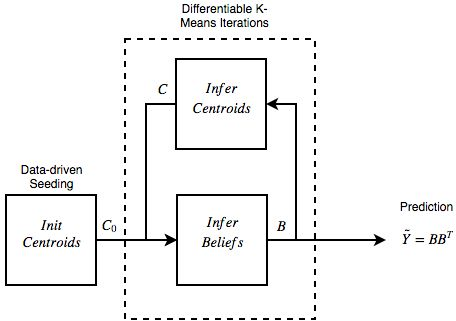
\includegraphics[width=0.7\textwidth]{imgs/dkmpp.jpg}
\caption{\label{fig:frog}Block diagram for clustering module.}
\end{figure}
As recalled, the original purpose of our algorithm was to learn parameters for an embedding function, s.t data embedded under it will yield good clustering performance, when clustered via algorithms which seek to minimize the K-Means objective. For this end we need the clustering inference to be a differentiable function, so that gradients could be back-propagated.
Let us notice that in Loyd's algorithm, the only part in the update steps which isn't differentiable is the assignment of datapoints to clusters, for which an $argmin$ needs to be computed. This operation is clearly not differentiable, and so instead we propose to use a $softmin$. This operation turns our assignments into soft-decisions, which we denote as beliefs, and represent via a row-stochastic belief matrix $B\in \reals^{n,k}$
The equations for the relaxed Voronoi updates are, in matrix notation: 
\begin{equation*} 
\begin{aligned}
& B_{t+1} = softmin(dist\_mat(X,C_{t})) \\
& C_{t+1} = diag((B_{t+1}^T X)\vec{1} )^{-1}(B_{t+1}^T X)
\end{aligned}
\end{equation*}
Where $dist_mat$ is defined as.. TODO 
,and $diag$ is defined by taking a vector as input, and giving a square matrix whose main diagonal is that vector as output.
For further clarity, let us view these updates in pseudo-code and describe the meaning of each line:
%todo: change name to deep expectation maximization
\begin{algorithm}[H]
\caption{Deep K-Means++}
\begin{algorithmic}[1]
	\State \textbf{Input:} Embedded Data $\widetilde{X}$, Number of clusters $k$, Unroll depth $l$. 
    \State $C_0 \gets $ Deep K-Means++ Init($\widetilde{X}$) \Comment{Data-driven centroid initialization}
    \For{i = 1 to l}
    \State $B_i \gets $ Infer-Beliefs($\widetilde{X},C_{i-1},\beta$)
    \State $C_i \gets $ Infer-Centroids($\widetilde{X},B_{i-1}$)
    \EndFor
    \State \Return $B_{l} B_{l}^{T}$
\end{algorithmic}
\end{algorithm}
\begin{algorithm}[H]
\caption{Get Distance Matrix}
\begin{algorithmic}[1]
	\State \textbf{Input:} Two matrices $A\in\mathbb{R}_{n,d},B\in\mathbb{R}_{k,d}$, with same row dimensionality
    \State $D \gets (A\odot A)1_{d,k}-2AB^{T}+((B\odot B)1_{d,k})^{T}$ \Comment{Using lin. alg. identity: $||u-v||^2=||u||^2-2<u,v>+||v||^2$}
    \State Return $D$ \Comment{$ij$'th cell stores squared euclidean distance between $i$'th row of $A$ and $j$'th row of $B$}
\end{algorithmic}
\end{algorithm}
\begin{minipage}[t]{8cm}
  \vspace{0pt}  
  \begin{algorithm}[H]
    \caption{Infer-Beliefs}
    \begin{algorithmic}[1]
    \State \textbf{Input:} Data Matrix $X$, Centroid Matrix $C$
    \State $dist\_mat \gets get\_distance\_matrix(X,C)$
    \State \Return $softmin(dist\_mat)$
    \end{algorithmic}
  \end{algorithm}
\end{minipage}%
\begin{minipage}[t]{7cm}
  \vspace{0pt}
  \begin{algorithm}[H]
    \caption{Infer-Centroids}
    \begin{algorithmic}[1]
    \State \textbf{Input:} Data Matrix $X$, Belief Matrix $B$
    \State $cluster\_sums \gets B^T X $
    \State $cluster\_sizes \gets cluster\_sums\dot\vec{1} $
    \State $normalizer \gets diag(cluster\_sums)^{-1}$
    \State \Return $ normalizer\times{cluster\_sums}$
    \end{algorithmic}
  \end{algorithm}
  
\end{minipage}


The clustering module's pseudo-code is described at algorithm 2, and is based on a differentiable formulation of the K-Means++ algorithm. As mentioned above,

This clustering module represents the clustering using a set of underlying cluster centroids, which induce the soft-assignment (which we will denote by the term beliefs) of data points to clusters. The belief vector for each data point is given by applying a softmin operation over the vector of euclidean distances between that data point and the existing centroids. We use a softmin instead of an actual argmin so that our cluster inference will be a differentiable function, and will thus yield to end-to-end gradient descent updates.

\section{Differentiable Centroid Sampling}
for the gradient signal to be helpful, we need the clustering inference to work properly. If the data is embedded correctly, i.e such the the global optimal cluster
In order for the learning process not to be derailed by wrong clusterings (i.e, the gradient update will move the embedding parameters in a direction such that the labeled data will be better clustered under a bad local minima in the clustering output space)
\begin{algorithm}[H]
\caption{Deep K-Means++ Init}
\begin{algorithmic}[1]
	\State \textbf{Input:} Data matrix $X$, Number of desired clusters $k$.
    %\bindent
    \State $C_0 \gets X_0$ \Comment{assign first centroid to be arbitrary data point}
    \For{i = 1 to k-1}
    	\State $C \gets [C_0,..,C_{i-1}]$
    	\State $D \gets get\_dist\_mat(X,C)$ \Comment{ $ij$'th cell stores squared euclidean distance between $i$'th data point and $j$'th centroid}
        \State $\widetilde{D} \gets softmin(D)\odot D$ \Comment{apply softmin over every row, and multiply element-wise with $D$ }
    	\State $\pi \gets \frac{\widetilde{D}\vec{1_{i}}}{\vec{1_{n}}\widetilde{D}\vec{1_{i}}}$ \Comment{sum over rows and normalize. $\pi$ thus represents a discrete distribution}
    	\State $\vec{q} \gets gumbel\_softmax\_sampling(\pi)$ \Comment{relaxed one-hot vector indicating $i$th centroid picked} 
    	\State $C_i \gets \vec{q}X$
    \EndFor
    \State $C \gets [C_0,..,C_{k-1}]$
	\State \Return $C$
	%\eindent
\end{algorithmic}
\end{algorithm}
We now describe how we implement {\it{k-means++}}'s centroid initialization as a differentiable layer in a neural network.\\
As in {\it{k-means++}} our algorithm proposes centroids iteratively. At the first iteration, we simply propose an arbitrary data point. At the $t+1$'th iteration, $t$ centroids, denoted as $\{c_i\}_{i=1}^{t}$, have already been proposed. 
A matrix $D$ of size $[n,t]$ can thus be built, such that $A_{i,j} =  ||x_i-c_j||^2$. By taking a soft-min over $D$'s rows and normalizing the result to 1, we have an approximation for the probability vector, whose $i$'th entry is  \\
\subsection{Gumbel-Softmax Sampling}
%explanation of gumbel softmax sampling. gumbel distribution, etc
Gumbel-Softmax Sampling is a differentiable version of sampling from a discrete probability distribution. This technique allows defining neural networks with layers that act as discrete samplers. 
TODO: add when this is usefull (gans,etc..)
Notice that it is not possible to implement such layers in neural networks without any output smoothing, since sampling from a discrete distribution is inherently non-differentiable.\\
The sampling layer takes as input a vector of probabilities $\{p_i\}_{i=1}^{n}$, and outputs a distribution over possible 

The method uses the following key fact from probability theory:
\begin{thm}
(Gumbel Sampling) Let $p_1,...,p_n \in \Delta_n$ be $n$ numbers on the $n$-simplex, and denote by $D$ a random variable over $[n]$, distributed by $P[D=i]=p_i$.\\
Let $Z$ be a random variable over $\reals$ with the following probability density function: $f(z) = e^{-z+e^{-z}}$.\\
Then, the random variable $argmax_{i\in[n]}\{Z\cdot p_i\}$ has the same distribution as $D$.
\end{thm}
\begin{proof} 
Let $\{x_i\}_{i=1}^{n}$ be $n$ real numbers s.t $\forall i\in[n]: p_{i} = \frac{e^x_i}{\sum_{k'}}$
\end{proof}
\begin{algorithm}[H]
\caption{Gumbel-Softmax Sampling}
\begin{algorithmic}[1]
	\State \textbf{Input:} A discrete probability distribution $\pi = \{p_i\}_{i=1}^{n}$
    %\bindent
    \State sample $\vec{z}\in \mathbb{R}^n$, where each coordinate is sampled according to the Gumbel distribution: $p(z) = e^{-(z+e^{-z})}$
    \State $\widetilde{\pi} \gets \pi \odot \vec{z}$ \Comment{multiplicatively perturbed values}
    \State Return $softmax(\widetilde{\pi})$
    %\eindent
\end{algorithmic}
\end{algorithm}
\chapter{Experiments}
\label{experiments}

\begin{figure}
\centering
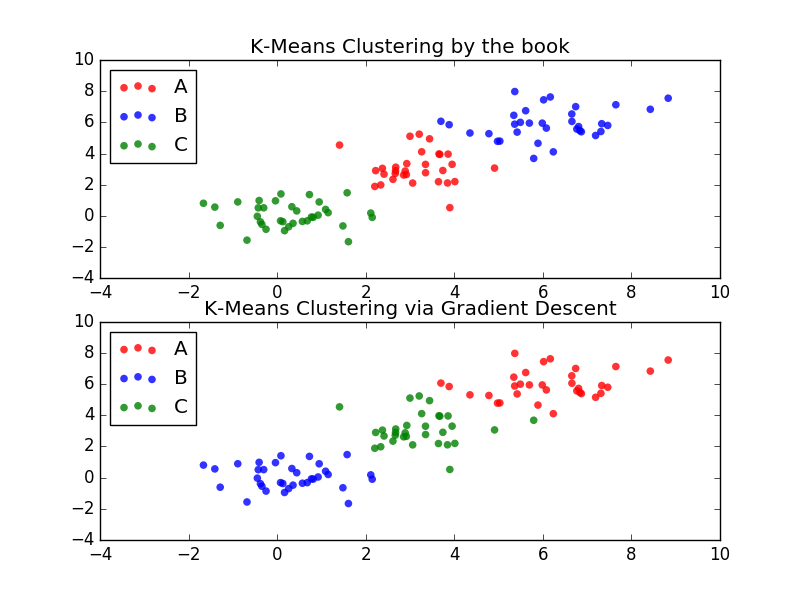
\includegraphics[width=0.7\textwidth]{imgs/gd_clust_good_attempt.png}
\caption{\label{fig:gd_clust_good} Example of a successful K-means clustering via Gradient Descent over the logits of cluster membership probabilities.}
\end{figure}
\section{Experiments with synthetic data}
\subsection{Learning a linear projection}
In this subsection we describe our experiments with learning the parameters of a simple embedding function, namely a linear projection $f:\R^n \rightarrow \R$, whose parameters should be learned.\\
The performance of an end-to-end clustering algorithm relies on many design choices and factors, and how they relate to the specific problem at hand.\\
In our experiments we examined the following factors:\\
\begin{itemize}
\item Clustering algorithm to be unrolled.  
\item Number of iterations which the clustering algorithm performs.
\item Various clusterer-specific hyperparameters, such as the bandwidth for the EM-clusterer, and the learn-rate and decrease schedule for the Differentiable-K-Means. 
\end{itemize}
We examined these and related factors on the following synthetic data sets:\\
I) Co-linear Gaussian Clusters\\
In this data set, the data is simply generated by a mixture of Gaussians, whose means are co-linear. The cluster membership for the data points correspond to the Gaussians which they are sampled from. \\
The Gaussians in this data set have isotopic covariance matrices, and since their means are co-linear, we know that the optimal linear projection parameters should be proportional to the parameters of the line which connects the Gaussians means.\\ % explain why this is the best?
An example for $n=3$ is portrayed at Figure x.\\
Anecdote: If you learn a linear projection for the ambiguous gaussians (placed at $10*unit_square$) plus a scaling factor, then using the EM clusterer, the scaling factor is pushed down. If you shrink the data by 0.1, the scale factor is pushed up. It stops changing at about $0.2$ times original data. why is that so?
\begin{comment}
\begin{figure}[h]
\begin{subfigure}{0.5\textwidth}
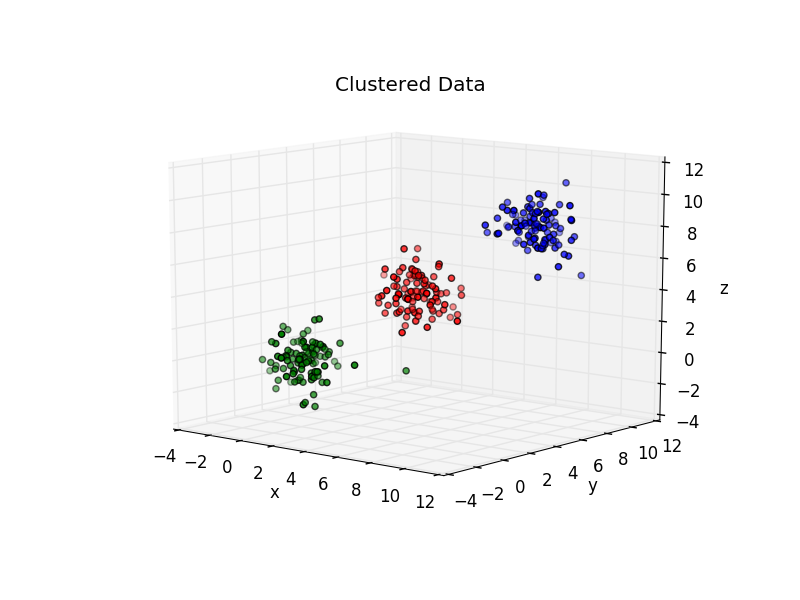
\includegraphics[width=0.9\linewidth, height=5cm]{imgs/figure_2.png} 
\caption{Co-Linear Gaussians}
\label{fig:subim1}
\end{subfigure}
\begin{subfigure}{0.5\textwidth}
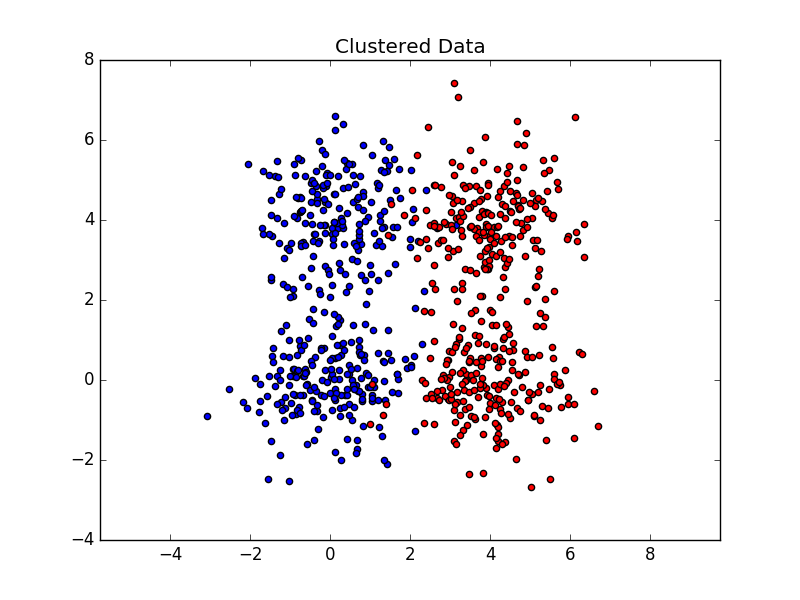
\includegraphics[width=0.9\linewidth, height=5cm]{imgs/ambiguous.png}
\caption{Ambiguous Gaussians}
\label{fig:subim2}
\end{subfigure}
\caption{Caption for this figure with two images}
\label{fig:image2}
\end{figure}
 \end{comment}
II) Ambiguous Gaussians % should a different term be used?

\section{Experiments With Real-World Data}
\subsection{Datasets}
\subsection{Experimental Protocol}
\subsection{Model Selection}
There were different design choices to pick from when implementing our algorithm.\\
Learning rate was selected by taking the largest rate power of $0.1$ for which the training process was stable.
The size $n$ of mini-batches was taken to be the largest that could fit in our GPU.  
Other choices were:
\begin{itemize}
\item Unroll depth $l$, i.e number of clustering steps 
\item Number $k$ of clusters per mini-batch.
\item Temperature for exponents in Gumbel Sampling and EM. 
\end{itemize}
Since the datasets we used do not have an official validation split used by other works, we introduced our own splits. For the CUB and Cars datasets we split the train data to two halves with mutually exclusive categories, and use holdout validation on one of them. For both datasets the optimal design choice was the same ($l=3$,$k=10$), and the results we report are with these models trained on the entire available train data.\\
For the Online Products dataset,...

%step 0: show that init 2 still outperforms other inits. we have plot for this

at first we checked which lr's are ok for the training to converge. this led us to 1e-5,1e-6.
% data for next paragraph in dir first_try
then we checked which bandwith params to use. at first we did this with lr=1e-5. this showed overfitting.

later we tried with lr=1e-6, which did not result in overfitting. this is interesting- shows a qualitative difference in models.

\begin{figure}
\centering
\includegraphics[width=0.7\textwidth]{imgs/em_bw.png}
\caption{\label{fig:gd_clust_good} Model selection for which EM bandwidth to use.}
\end{figure}
Seems we didn't reach the best yet, so let's take even higher bandwidths:

\begin{figure}
\centering
\includegraphics[width=0.7\textwidth]{imgs/em_bw_second_try.png}
\caption{\label{fig:gd_clust_good} Model selection for which EM bandwidth to use.}
\end{figure}

Best is bw=1.
Let's check now for temperature in the Gumbel sampling phase, and for the soft-min operation's bandwidth.

\begin{figure}
\centering
\includegraphics[width=0.7\textwidth]{imgs/gumbel_temp.png}
\caption{\label{fig:gd_clust_good} Model selection for which temperature to use at Gumbel sampling phase.}
\end{figure}

\begin{figure}
\centering
\includegraphics[width=0.7\textwidth]{imgs/softmin_bw.png}
\caption{\label{fig:gd_clust_good} Model selection for which bandwidth to use at soft-min step.}
\end{figure}

when checking bw selection for lr=1e-6 we see that best gumbel temp and softmin_bw are 1.

What happens when we combine these different choices together?

\begin{figure}
\centering
\includegraphics[width=0.7\textwidth]{imgs/combined_argmax_bad.png}
\caption{\label{fig:gd_clust_good} Combination of different model choices yields bad design.}
\end{figure}

Lets use the argmax then. that is when softmin_bw = 1, and the rest is the same
Now lets give it a total run with nmi loss as well


\subsection{Implementation Details}
\subsection{Results}
\subsection{General Details}
Following the experiments described at zemel17 song16, we test our approach on three known datasets:\\
\begin{itemize}
\item Caltech-UCSD Birds 200 \cite{WahCUB_200_2011}
\item Stanford Cars Dataset
\item Stanford Products Dataset
\end{itemize}
Each dataset consists of images which come from some shared context (i.e images of birds, cars or consumer products). The images in each dataset are further categorized into classes (E.g "Laysan Albatross" for birds, "2012 Tesla Model S" for cars, etc.) where images in the same class are considered semantically similar.
We split the datasets to a train and test set according to the splits described in Zemel17,Song16. At train time, mini-batches of images are sampled, and a clustering matrix over the sampled images is predicted. The $L_2$ difference between the prediction and the ground-truth matrix is used cost function.\\
The code for our experiments was written in Tensorflow \cite{greenwade93} version 1.8.0. A link to the publicly available git repository is listed below.\footnote{Link: \url{https://github.com/DanielCarmon/msc_project}}
\subsubsection{Depth of K-Means unrolling}
In our experiments different unroll depths $T\in\{1,3,5,10\}$ are tested. In the case where $T=1$, we simply output $BB^t$ as the prediction, where $B\in\mathbb{R}^n,k$ is the belief matrix for when the centroids are those initially sampled by the differentiable centroid sampling module described above. 
In the results section it is seen that deeper doesn't necessarily mean better, and that usually there is a "sweetspot", or optimal unroll depth $T$ for learning through K-Means optimization.

\subsubsection{Embedding Function}
As an embedding function $f:D\rightarrow \mathbb{R}^d$, we use the Inception-v3 \cite{greenwade93} architecture, with parameters pre-trained on the ImageNet\cite{greenwade93} dataset. As in Zemel17, song16, we removed the softmax operation at the last layer of the network, and added a linear layer. The output dimentionality $d$ of our linear layer is set to be the number of train classes for the first two datasets, and $512$ for the Products dataset, where the number of train classes is larger than $10^4$.\\

\subsubsection{Training Details}
% general pipeline
At train time we use batches of $n=100$ images per update step, with a ground-truth clustering matrix $Y\in R^{n,n}$. These images are sampled from $k\in{\{5,10,20\}}$ different classes, with each class contributing $n/k$ images to the batch. The $k$ class indices too are sampled at each iteration from a pool of classes whose images constitute the train data. Results for different values of $k$ are shown below.\\
% trajectory gradients
When training with differentiable clusterers that have intermediate beliefs (i.e when the unroll depth of the clusterer is greater than $1$), we use "auxillary gradients" by adding the loss for intermediate beliefs to the loss function we optimize over. This trick appears in previous deep learning works as well. E.g in \cite{greenwade93}, where the original Inception-v3 network was trained on ImageNet, "auxillary classifier" layers are maintained at train time, and their loss is added to the total loss function of the network. At test time, these classifiers are discarded. Using these "auxillary gradients" in our case favors embeddings who's clustering under K-Means++ doesn't just converges to a good local optima, but also does so quickly. Another way in which this trick benefits the training process is that it helps to alleviate the vanishing gradient problem\cite{greenwade93}, which occurs as unroll depth is increased.\\ % does it really occur?
Data pre-processing was done in the following way. Each image was first reshaped to shape $[299,299,3]$, in order to fit the Inception network's fixed input size. Afterwards the pixel intensities of each image were linearly scaled to $[0,1]$. For data augmentation, we used a single horizontal flip per image.\\
The following hyperparameters were used in our experiments. The bandwidth for the softmax at the differentiable clusterer's E-step is $1e-1$. We used the Adam \cite{} optimizer with a base learn rate of $1e-6$ to train the deep network's parameters.
We trained our models for $5e+4$ steps, which on a standard work station with a 3GHz 16-Core PC with 125GB RAM and a GeForce GTX TITAN X GPU with 13GB RAM took about 1 day to complete. 
\subsubsection{Testing Details}
At test time, the embedding function learned during training is used to embed the test data. 
The original (i.e non-differentiable) K-Means++ algorithm is then used to cluster the embedded test data, and the Normalized Mutual Information (NMI) \cite{greenwade93} is then used as a difference measure between the K-Means++ clustering over the embedded data and the ground-truth clustering.\\
In our experiments we used $\it{sklearn}$'s \cite{greenwade93} implementation for K-means++.
We tested the K-Means++ clustering every 100 parameter updates, in order to see how the NMI score for the learned embedding changes across training. We present results for the train data and the test data. % should we?
In the first two datasets, the classes in the train and test data are disjoint, although coming from a shared context (all being images of birds or cars). In the third dataset (Stanford Products), where an average class has about $5.3$ images, some classes occur in both data splits and some don't. In all cases, the learner must be able to generalize from classes seen during training to previously unseen classes. 

\subsection{CUB Dataset}
The CUB Dataset is comprised of 200 classes of different birds. Each class contains about 60 instances belonging to a single species. We sp lit the data to have the first 100 classes (5,864 images) for training, and the last 100 classes (5,924 images) for testing.
\subsubsection{Training Details}
...
\subsubsection{Results}
After every 100 parameter updates, we tested how well can the newly represented data be clustered, both for the train data and the test."Goodness of clustering" was measured via normalized mutual information. The following table shows both for train and test data how close with regard to ground truth were the new representations clustered.\\
\begin{figure}[h!]
\centering
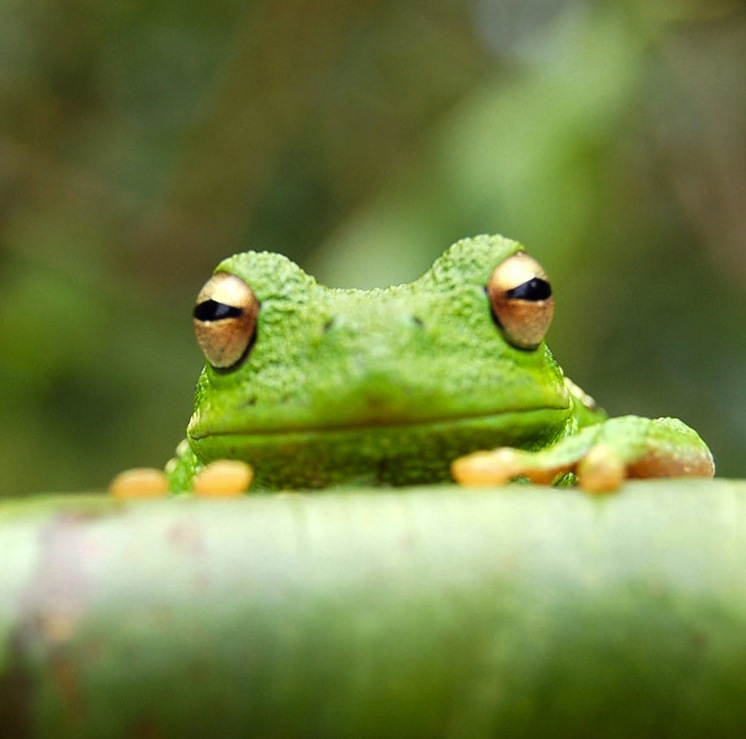
\includegraphics[width=0.3\textwidth]{imgs/frog.jpg}
\caption{\label{fig:frog}placeholder for image.}
\end{figure}
TODO: Add image that shows this. When done doing design choices elimination, train the best.
The following table summarizes the NMI score of previous benchmarks with addition to ours:
\begin{table}[h!]
\centering
\begin{tabular}{l|r}
Method & NMI \\\hline
Triplet s.h. (Schroff et al., 2015) & 55.38 \\
Lifted struct. (Song et al., 2016) & 56.50 \\
Npairs (Sohn, 2016) & 57.24 \\
Facility loc.(Song et al., 2017) & 59.23 \\
Spectral clust. (Zemel et al., 2017) & 59.16 \\
Ours & 60+ 
\end{tabular}
\caption{\label{tab:score compare} NMI evaluation on the Birds (CUB-200-
2011) dataset.}
\end{table}
\subsection{Stanford Cars Dataset}
Description of dataset goes here
\subsubsection{Training Details}
\subsubsection{Results}
\subsection{Ablation Studies}
We perform the following ablation studies on the Caltech-UCSD Birds-200-2011 dataset. We measure the NMI score of different variations in the architecture we proposed above. The variations we examined are difference in depth of the clustering inference module (i.e, how many belief update iterations occurred) and difference in number of clusters per training batch (i.e, how many bird categories where seen during each training iteration). There are existing trade-offs for each of these design choices. A deeper clustering inference module will give more accurate results, but may dilute the gradient signal such that learning is dampened. For the number of clusters per batch, a high number of seen categories in each batch may help reach a representation which will generalize (see discussion on ZSL in \ref{e2e_rep_learn}) better, yet on the other hand a too high number of categories will emphasize intra-cluster differences, while at the extreme end (when $k=n$) the supervision signal is degenerated to simply be the identity matrix. For both these design choice dimensions it seems from the following ablation studies that there is a "sweet-spot" somewhere between the extreme values. The variation which reached the highest NMI score over the test data isn't the model that was suggested by evaluating the different variation's clustering over the first 100 categories, and thus we did not report it's score (~0.62 NMI) when comparing our approach to other works. 

\iffalse
\begin{figure}[h!]
\centering
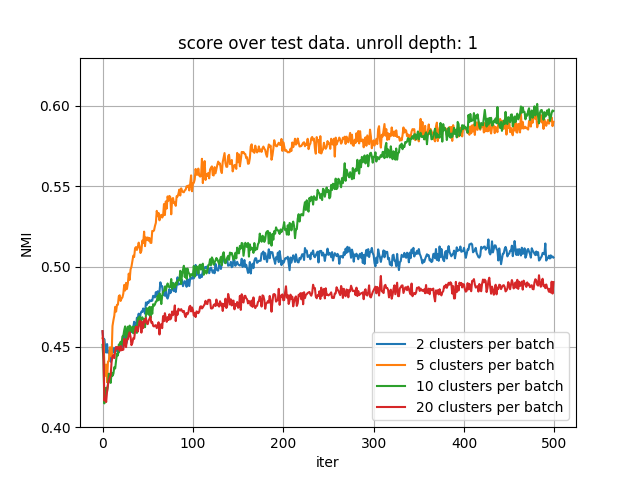
\includegraphics[width=1\textwidth]{imgs/cub_test_500/square/depth1.png}
\caption{\label{fig:cub_test_500} NMI Test scores for architecture with single belief update step.}
\end{figure}
\begin{figure}[h!]
\centering
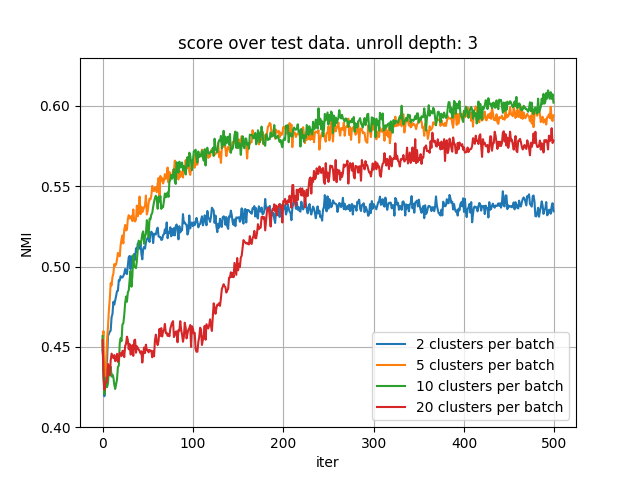
\includegraphics[width=1\textwidth]{imgs/cub_test_500/square/depth3.png}
\caption{\label{fig:cub_test_500} NMI Test scores for architecture with three belief update steps.}
\end{figure}
\begin{figure}[h!]
\centering
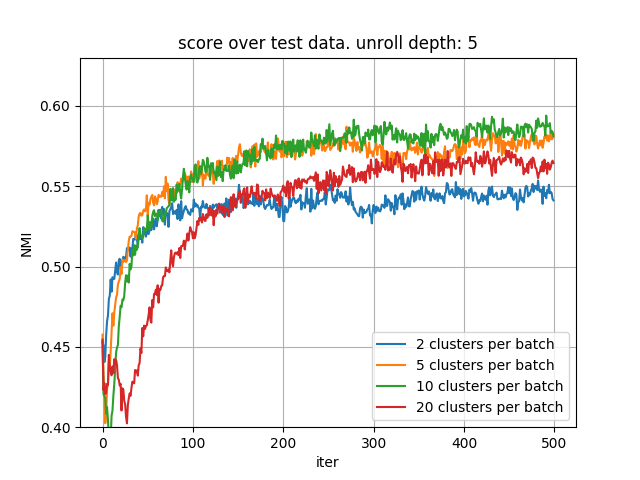
\includegraphics[width=1\textwidth]{imgs/cub_test_500/square/depth5.png}
\caption{\label{fig:cub_test_500} NMI Test scores for architecture with five belief update steps.}
\end{figure}
\begin{figure}[h!]
\centering
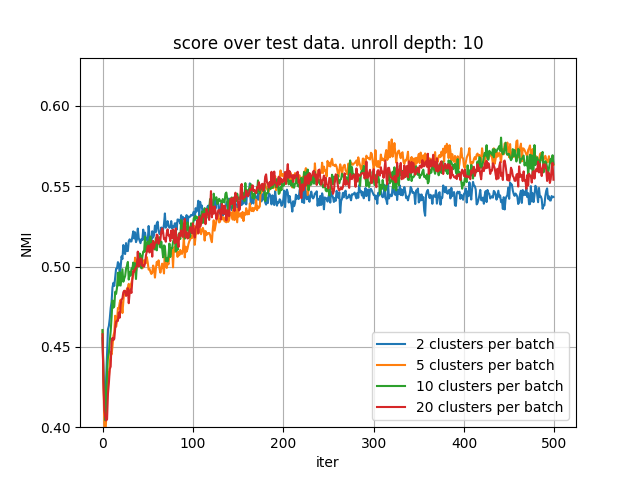
\includegraphics[width=1\textwidth]{imgs/cub_test_500/square/depth10.png}
\caption{\label{fig:cub_test_500} NMI Test scores for architecture with ten belief update steps.}
\end{figure}
\begin{figure}[h!]
\centering
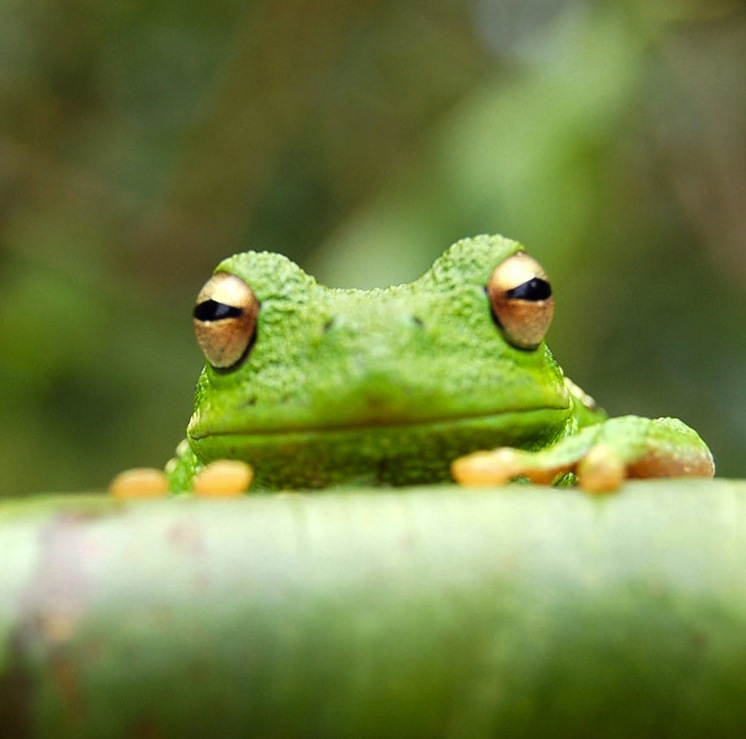
\includegraphics[width=0.3\textwidth]{imgs/frog.jpg}
\caption{\label{fig:frog}placeholder for image.}
\end{figure}
TODO: Add image that shows this. When done doing design choices elimination, train the best.
The following table summarizes the NMI score of previous benchmarks with addition to ours:
\begin{table}[h!]
\centering
\begin{tabular}{l|r}
Method & NMI \\\hline
Triplet s.h. (Schroff et al., 2015) & 53.35 \\
Lifted struct (Song et al., 2016) & 56.88 \\
Npairs (Sohn, 2016) & 57.79 \\ 
Facility loc. (Song et al., 2017) & 59.04 \\
Spectral clust. (Zemel et atl., 2017) & 64.25 \\
\end{tabular}
\caption{\label{tab:score compare} NMI and Recall@K evaluation on the Cars196 dataset.}
\end{table}
\subsection{Stanford Products Dataset}
Description of dataset goes here
\subsubsection{Training Details}
\subsubsection{Results}
\begin{figure}[h!]
\centering
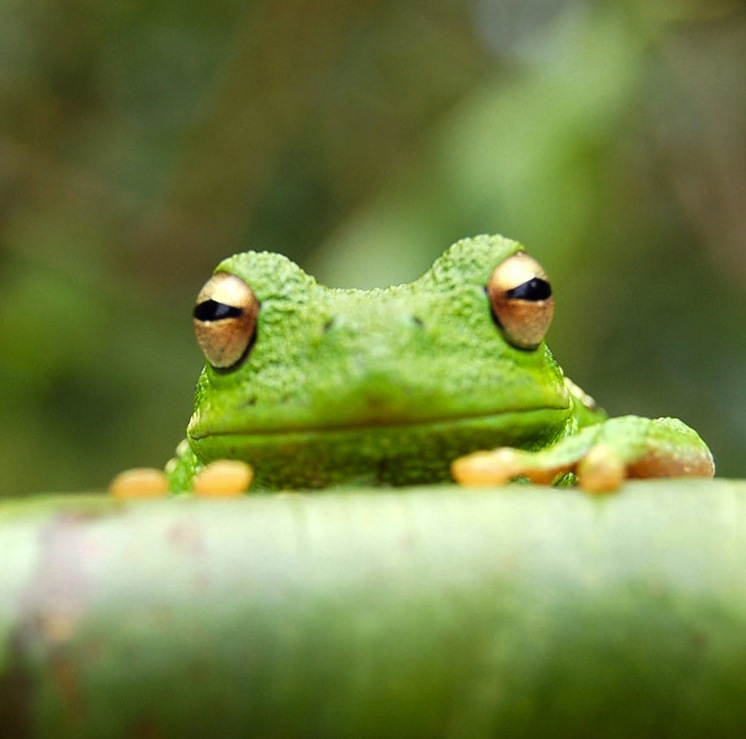
\includegraphics[width=0.3\textwidth]{imgs/frog.jpg}
\caption{\label{fig:frog}placeholder for image.}
\end{figure}
TODO: Add image that shows this. When done doing design choices elimination, train the best.
The following table summarizes the NMI score of previous benchmarks with addition to ours:
\begin{table}[h!]
\centering
\begin{tabular}{l|r}[h!]
Method & NMI \\\hline
Triplet s.h. (Schroff et al., 2015) & 89.46 \\
Lifted struct. (Song et al., 2016) & 88.65 \\
Npairs (Sohn, 2016) & 89.37 \\
Facility loc.(Song et al., 2017) & 89.48 \\
Spectral clust. (Zemel et al., 2017) &  89.40 \\
Ours & ?
\end{tabular}
\caption{\label{tab:score compare} NMI evaluation on the Products (Stanford
Online Products) dataset.}
\end{table}


\begin{comment}
\subsubsection{Effect of Unrolling Depth}
\subsubsection{Effect of Centroid Initialization Method}
\begin{figure}[h!]
\centering
\includegraphics[width=0.3\textwidth]{centroid_init_comparison.png}
\caption{\label{fig:init_comparison} Comparison of NMI scores when trained using different centroid initialization methods.}
\end{figure}
\end{comment}

\fi


%\input{inference.tex}
%Sets as inputs to Neural Networks}
Many computational tasks require as an input a \textit{set} of elements, i.e an invariance over any permutation of these elements is required from an algorithm which solves the said computational task.\\
Examples for such tasks are quite vast (e.g computation of population statistics, and combinatorical problems such as the Knapsack Problem \cite{gareyjohnson79}), and the task of clustering demands this invariance as well.\\
todo: add hand-written-circuit vs learned circuit part.
\subsection{Permutation-invariant Neural Networks}
Recently, \cite{zaheer17} proposed the following nessecary and sufficient condition for a neural architecture to be permutation invariant by design.\\
todo: describe architecture condition
\subsection{Permutation-invariance and permutation-equivariance}
An alternative request from an architecture that realizes a function over sets, is to work with a representation which is permutation-\textit{equivariance} instead of permutation-\textit{invariant}.\\
We say that a function $f\in X^n\rightarrow Y^n$ is permutation-equivariant if the following holds:\\
$\forall\pi\in S_n: f(x_\pi(1),...,x_\pi(n))=(f(x))_\pi(1),...,(f(x))_\pi(n)$\\
In other words: a function is permutation-equivariant if permuting the input = permuting the output by the same permutation. \\ 
\cite{zaheer17} discusses permutation-equivariance, yet only for a limited function class, namely neural-networks with a single weight layer.\\
Based on their work with permutation-invariance let us describe now a necessary and sufficient condition for a neural-network architecture to be permutation-equivariant.\\
We claim the following:\\
Lemma: \\
A neural-network $\Phi$ is permutation-equivariant iff $f$ can be factored in the following way:\\
$ f(x_1,...,x_n) = \Psi(x_1,DS(x_{-1})),...,\Psi(x_n,DS(x_{-n}))$\\
Where $DS$ is a permutation-invariant architecture such as the one purposed at \cite{zaheer17}.\\
Proof idea: \\
The equivariance condition holds iff for every $i\in[n]$, $f(x)_i$ doesn't depend on the ordering of $x_{-i}$. \\ Therefore it is a function of two inputs: $x_i$, and $x_{-i}$ as a $\it{set}$. \\
This factorization is necessary in the sense that if a function $f$ has the p.e property, then there is a network with the above architecture which implements it.\\ % up to epsilon
In the task of classification, usually one is learning a classification rule $\Psi:X\rightarrow Y$. This fits in our lemma with $\Psi$ as defined above ignoring it's second argument. \\
Yet in the task of clustering, such a $\Psi$ may not be sufficient, and context is usually be crucial. \\ E.g clustering 4 points on a randomly sampled 2D rectangle to two clusters, in attempt to minimize the Kmeans loss. One cannot solve this task by learning a fixed function from a single point to cluster identity.\\
We later describe experiments with learning such "hollistic" clustering networks. 
\chapter{Discussion}
\label{sec:discussion}  

Generally in structured prediction, and specifically in dependency grammars, obtaining annotated data requires expensive human expertise. However, unlabeled data is widely available on the web. Therefore, semi-supervised methods are of high interest in these fields.

In this work, we presented a general semi-supervised approach for injecting well-known structural properties of dependency parsing, \textit{acyclicity} and \textit{projectivity}. This is done by differentiable loss function, punishing for violation of these constraints on unlabeled data. To the best of our knowledge, this is the first work that directly considers the model's continuous scores, rather than discrete outputs. Our method is well-suited for any first-order graph-based parser, and is independent of the underlying scoring mechanism.

We were able to show improvement over a supervised baseline both in prediction performance and structural generalization\footnote{Namely, increase of valid structures during test time}. In addition, we analyzed a greedy approach for decoding.
We also demonstrated how this procedure benefits from the improvement in structural generalization.

We leave two natural extensions of this method for future work. The first considers designing strong discriminators to catch (perhaps unknown) phenomenas occurring in dependency trees. Architectures of such discriminators may vary and have not been addressed yet. Note that discriminators can also be combined with the inference procedure, by outputting structures with high likelihood\footnote{In other words, structures with high scores from the discriminator}.

Extending our method to the discrete case is also of interest, since it is not always possible to come up with efficiently computable differentiable loss functions correlated to high-order constraints.

\iffalse
The key theoretical question in deep learning is why it succeeds in finding good models despite the non-convexity of the training loss. It is clear
that an answer must characterize specific settings where deep learning provably works. Despite considerable recent effort, such a case has not been shown. Here
we provide the first analysis of a non-linear architecture where gradient descent is globally optimal, for a certain input distribution, namely Gaussian. Thus our specific
characterization is both in terms of architecture (no-overlap networks, single hidden layer, and average pooling) and input distribution. We show that  
learning in no-overlap architectures is hard, so that some input distribution restriction is necessary for tractability. Note however, that it is certainly possible
that other, non-Gaussian, distributions also result in tractability. Some candidates would be sub-Gaussian and log-concave distributions.

Our derivation addressed the population risk, which for the Gaussian case can be calculated in closed form. In practice, one minimizes an empirical risk. Our experiments in \secref{nonoverlap_experiments} suggest that optimizing the empirical risk in the Gaussian case is tractable. It would be interesting to prove this formally. It is likely that measure concentration results can be used to get similar results to those we had for the population risk (for use of such tools see \cite{mei2016landscape,xu2016global}).

Convolution layers are among the basic building block of neural networks. Our work is among the first to analyze optimization for these. The architecture we study is similar in structure to convolutional networks, in the sense
of using parameter tying and pooling. However, most standard convolutional layers have overlap and use max pooling. In \secref{sec:nets_with_overlap} we provide initial results for the case of overlap, showing there is hope for proving 
optimality for gradient descent with random restarts. Analyzing max pooling would be very interesting and is left for future work. 

Finally, we note that distribution dependent tractability has been shown for intersection of halfspaces \cite{klivans2009baum}, which is a non-convolutional architecture. However, these results do not use gradient descent. It would be very interesting to use our techniques to try and understand gradient descent for the population risk in these settings.    
\fi

\newpage

\bibliographystyle{alpha}
\bibliography{Zotero}



\includepdf[pages=-]{heb_abstract.pdf}


\includepdf[pages=-]{cover_heb.pdf}

\end{document}
